\documentclass[11pt,a4paper,titlepage,draft]{article}
\usepackage[utf8]{inputenc}
\usepackage[greek]{babel}
\usepackage{amsmath}
\usepackage{amsfonts}
\usepackage{amssymb}
\usepackage{commath}
\usepackage{xcolor}
\usepackage{hyperref}
\usepackage[skins,theorems]{tcolorbox}
\usepackage{titlesec}
\usepackage{circuitikz}
\usepackage{pgfplots}
\usepackage{gfsartemisia}
\usepackage{mathtools}
\usepackage[makeroom]{cancel}
\usepackage{mathrsfs}


\usetikzlibrary{arrows.meta}

\usepackage[left=2cm,right=2cm,top=2cm,bottom=2cm]{geometry}

\makeatletter
%\newcommand{\attnboxed}[1]{\textcolor{red}{\fbox{\normalcolor\m@th$\displaystyle#1$}}}
\makeatother
\tcbset{highlight math style={enhanced,colframe=red,colback=white,%
  arc=0pt,boxrule=1pt,shrink tight,boxsep=1.5mm,extrude by=0.5mm}}
\newcommand{\attnboxed}[1]{\tcbhighmath[colback=red!5!white,drop fuzzy shadow,arc=0mm]{#1}}
\titleformat{\section}{\bf\Large}{Κεφάλαιο \thesection}{1em}{}
\newtcolorbox{attnbox}[1]{colback=red!5!white,%
  colframe=red!75!black,fonttitle=\bfseries,title=#1}
\newtcolorbox{infobox}[1]{colback=blue!5!white,%
  colframe=blue!75!black,fonttitle=\bfseries,title=#1}
  
%\pgfplotsset{compat=1.12}

\title{Σημειώσεις Διαφορικές Εξισώσεις}
\date{2016, Εαρινό εξάμηνο}
\author{Καναβούρας Κωνσταντίνος \\ \textlatin{\url{http://users.auth.gr/konkanant}}}


\newtcbtheorem[number within=section]{theorem}{Θεώρημα}%
{colback=green!5,colframe=green!35!black,colbacktitle=green!35!black,fonttitle=\bfseries,enhanced,attach boxed title to top left={yshift=-2mm,xshift=-2mm}}{th}
\newtcbtheorem[number within=section]{defn}{Ορισμός}%
{colback=cyan!5,colframe=cyan!35!black,colbacktitle=cyan!35!black,fonttitle=\bfseries,enhanced,attach boxed title to top left={yshift=-2mm,xshift=-2mm}}{def}
\newtcbtheorem[number within=section]{exercise}{Άσκηση}%
{colback=gray!3,colframe=gray!35!black,colbacktitle=gray!35!black,fonttitle=\bfseries,enhanced,attach boxed title to top left={yshift=-2mm,xshift=-2mm}}{exc}

\begin{document}

\maketitle

%\tableofcontents

\newpage

\part{Σεβαστιάδης}
Χρήστος Σεβαστιάδης

\section{}

\begin{defn*}{Διαφορική εξίσωση}
Μια εξίσωση που αποτελείται από μια συνάρτηση και τις παραγώγους της
\end{defn*}

\paragraph{\textlatin{Langrange's}}
\(x',x'',x''',x^{(4)},\dots\)
\paragraph{\textlatin{Newton's}}
\(\dot{x}, \ddot{x}, \dddot{x}\)
\paragraph{\textlatin{Leibniz'}}
\(\od{x}{t}, \od[2]{x}{t}, \od[3]{x}{t}\)

\paragraph{}
\textit{π.χ.}
\[
x(t) \od[2]{x(t)}{t} + 2 \od{x(t)}{t}=x(t)\sin (t)
\]

\begin{defn}{Τάξη}{}
\textbf{Τάξη} ονομάζεται ο μεγαλύτερος \emph{βαθμός} παραγώγου που εμφανίζεται στην εξίσωση
\end{defn}

\begin{defn}{Βαθμός}{}
\textbf{Βαθμός} ονομάζεται η μεγαλύτερη \emph{δύναμη} παραγώγου που εμφανίζεται στην εξίσωση
\end{defn}


\section{Διαφορική εξίσωση 1ης τάξης}
\begin{defn*}{}
\[
\od{x}{t}=f(t,x)
\]
\end{defn*}

\paragraph{}

\subsection{Χωριζόμενες διαφορικές εξισώσεις}
Τυπική μορφή:
\[f(t,x) = \frac{-M(t,x)}{N(t,x)} = \od{x}{t}
\implies \underbrace{N(t,x)}_{N(x)} \dif x + \underbrace{M(t,x)}_{M(t)} \dif t = 0 \]

Αν δηλαδή τα \(N(t,x), \ M(t,x)\) εξαρτώνται μόνο από τα \(x\) και \(t\) αντίστοιχα, η εξίσωση ονομάζεται \textbf{χωριζόμενη}, και το αποτέλεσμά της μπορεί να βρεθεί με ολοκληρώματα:

\[
\int N(x) \dif x + \int M(t) \dif t = c
\]

\begin{exercise*}{2.1}
\[x \dif x - t^2 \dif t = 0 \]
\tcblower
\[ N(x) = x, \quad M(t)=-t^2 \]
\begin{align*}
&\int x \dif x + \int (-t^2) \dif t = c \implies \\
&\frac{1}{2} x ^ 2 - \frac{1}{3} t^3 = c \implies \\
&x = \pm \sqrt{\frac{2}{3} t^3 + 2c} \implies \\
&x= \pm \sqrt{\frac{2}{3} t^3 + \kappa } \\
\text{ με } \kappa =2c
\end{align*}
\end{exercise*}

\begin{exercise*}{2.2}
\[x' = x^2t^3 \]
\tcblower
\begin{align*}
&\implies \od{x}{t}=x^2t^3 \\
&\implies \frac{1}{x^2}\dif x - t^3 \dif t = 0 \\
&\implies \int \frac{1}{x^2}\dif x + \int (-t^3) \dif t = c \\
&\implies - \frac{1}{x} - \frac{t^4}{4} = c \\
&\implies - \frac{1}{x} = c + \frac{t^4}{4} \\
&\implies - \frac{4}{x} = 4c + t^4 \\
&\implies x = \frac{-4}{t^4 + \kappa}, \quad \text{με } \kappa = 2c
\end{align*}
\end{exercise*}


\begin{exercise*}{2.3}
\[x' = \frac{t+1}{x^4+1} \]
\tcblower
\begin{align*}
&\implies \od{x}{t}=\frac{t+1}{x^4+1} \\
&\implies (x^4+1) \dif x + (-t-1) \dif t = 0 \\
&\implies \int (x^4+1)\dif x + \int (-t-1) \dif t = c \\
&\implies \frac{x^5}{5} + x - \frac{t^2}{2} -t = c \\
\end{align*}
\end{exercise*}

Παρατηρούμε ότι, χωρίς αρχική συνθήκη, βρίσκουμε γενικές λύσεις ως αποτέλεσμα. Με τη χρήση μιας αρχικής συνθήκης, μπορούμε να βρούμε και την ειδική λύση της εξίσωσης.

\begin{exercise*}{2.4}
\[e^t \dif t - x \dif x = 0;\quad x(0)=1 \leftarrow \text{αρχική συνθήκη} \]
\tcblower
\begin{align*}
&\implies \int x \dif x + \int (-e^t) \dif t = c \\
&\implies \frac{x^2}{2} - e^t = c \\
&\implies x^2 = 2e^t + 2c \\
&\implies x^2 = 2e^t+ \kappa, \quad \text{με } \kappa = 2c
\end{align*}
Όμως \(x(0) = 1\), άρα:
\[
\begin{cases}
x^2 = 2e^t+ \kappa \\
x(0) = 1
\end{cases}
\implies x(0)^2 = 2e^0 + \kappa \implies \boxed{\kappa = -1}
\]
Επομένως τελικά:
\[
x^2=2e^t -1 \implies x = \pm \sqrt{2e^t-1} \implies \boxed{x=\sqrt{2e^t-1}}
\]

Η αρχική συνθήκη πράγματι επαληθεύει το αποτέλεσμα \(x\). Πρέπει όμως και \(x \in \mathbb R, \ 2e^t-1 \geq 0\).

Από τη διαφορική εξίσωση έχουμε \(x' = \frac{e^t}{x}\), άρα πρέπει \(2e^t - 1 > 0 \implies \boxed{t > \ln \frac{1}{2}} \).
\end{exercise*}




\[
\int_{x_0}^x N(x) \dif x + \int_{t_0}^t M(t) \dif t = 0, \quad x(t_0)=x_0
\]

\begin{exercise*}{2.5}
\[x \cos x \dif x + (1-6t^5) \dif t = 0; \quad t(\pi)=0 \]
\tcblower
\(x_0 = \pi,\ t_0 = 0\)
\begin{align*}
&\implies \int_\pi^x x \cos x \dif x +
\int_0^t (1-6t^5) \dif t = 0 \\
&\implies
\left. x \sin x \right|_\pi^x
+ \left. \cos x \right|_\pi^x + \left. (t-t^6) \right|_0^t = 0 \\
&\implies x \sin x + \cos x + 1 + t - t ^ 6 \\
&\implies \boxed{ x \sin x + \cos x + 1 = t - t^6 }
\end{align*}
\end{exercise*}

\subsection{Ομοιογενείς}
\[
f(t,x)= \frac{-M(t,x)}{N(t,x)}
\]

\begin{defn}{}{}
Αν \(\forall a \in \mathbb R: f(at,ax) = f(t,x)\), λέμε ότι η εξίσωση είναι \textbf{ομοιογενής}.
\end{defn}

\begin{theorem*}{}
Αν μια εξίσωση είναι ομοιογενής, μπορούμε να την λύσουμε μειώνοντάς/μετατρέποντάς την σε χωριζόμενη, εφαρμόζοντας το μαθηματικό κόλπο που ονομάζεται "αντικατάσταση μεταβλητής", δηλαδή, όπου \(u\) συνάρτηση:
\[
\boxed{
x=ut \implies \od{x}{t} = \od{u}{t}t+u
}\]
\end{theorem*}

\begin{exercise*}{2.6}
\[x' = \frac{x+t}{t} \]
\tcblower
\(\implies \od{x}{t} = \frac{x+t}{t}\), μη χωριζόμενη.
\[f(t,x) = \od{x}{t},\quad f(at,ax)= \frac{ax+at}{at} = \frac{x+t}{t} \text{ ομοιογενής}
\]
Θέτω \(x=ut, \ \od{x}{t}=\od{u}{t}t+u\), άρα η διαφορική εξίσωση γίνεται:
\begin{align*}
&\od{u}{t}t+u=\frac{ut+t}{t} \\ \implies&
\od{u}{t}t+u=u+1 \\ \implies&
t\od{u}{t} = 1 \\ \implies&
\frac{1}{t} \dif t - \dif u = 0 \text{ χωριζόμενη} \\ \implies&
\int \frac{1}{t} \dif t + \int (-1) \dif u = c \\ \implies&
\ln \abs t - u = c \\ \implies&
u = \ln \abs t -c \text{ με } c = - \ln \abs \kappa \\ \implies&
\boxed {u = \ln \abs{\kappa t}} \\ \implies&
\frac{x}{t} = \ln \abs{\kappa t} \implies
\boxed {x = t \ln \abs{\kappa t}}
\end{align*}
\end{exercise*}


\begin{exercise*}{2.7}
\[x' = \frac{2x^4+t^4}{tx^3} \]
\tcblower
\(\implies \od{x}{t} = \frac{2x^4+t^4}{tx^3}\), μη χωριζόμενη.
\[f(t,x) = \od{x}{t},\quad f(at,ax)= \frac{2(ax)^4+(at)^4}{(at)(ax)^3} = \frac{a^4 2x^4 + a^4t^4}{a^4tx^3} = \frac{2x^4+t^4}{tx^3} \text{ ομοιογενής}
\]
Θέτω \(x=ut, \ \od{x}{t}=\od{u}{t}t+u\), άρα η διαφορική εξίσωση γίνεται:
\begin{align*}
&
\od{u}{t}t+u=\frac{2(ut)^4+t^4}{t(ut)^3} \\ \implies&
\od{u}{t}t+u=\frac{2u^4 \cancel{t^4}+\cancel{t^4}}{u^3 \cancel{t^4}} \\ \implies&
\od{u}{t}t+u=\frac{2u^4+1}{u^3} \\ \implies&
\od{u}{t}t=\frac{2u^4+1}{u^3}-u=\frac{u^4+1}{u^3} \\ \implies&
\frac{u^3}{u^4+1} \dif u - \frac{1}{t} \dif t = 0 \text{ χωριζόμενη} \\ \implies&
\int \frac{u^3}{u^4+1} \dif u + \int \frac{-1}{t} \dif t = c \\ \implies&
\frac{1}{4} \ln (u^4+1) - \ln \abs t = c \\ \implies&
\boxed{u^4+1 = (\kappa t)^4} \text{ με } c = \ln \abs x \\
& x = ut \implies u = \frac{x}{t} \implies \left( \frac{x}{t} \right) ^ 4
+ 1 = (\kappa t )^4 \\ \implies&
\frac{x^4}{t^4}+1 = \kappa ^4 t^4 \\ \implies &
\boxed{x^4 = c_1t^8 - t^4} \text{ με } c_1= \kappa ^4
\end{align*}
\end{exercise*}


\begin{exercise*}{2.8}
\[x' = \frac{t^2+x^2}{tx}; x(1) = -2 \]
\tcblower
\(\implies \od{x}{t} = \frac{t^2+x^2}{tx}\), μη χωριζόμενη.
\[f(t,x) = \od{x}{t},\quad f(at,ax)= \frac{(at)^2+(ax)^2}{(at)(ax)} = \frac{\cancel{a^2}t^2+\cancel{a^2}x^2}{\cancel{a^2}tx} = \frac{t^2+x^2}{tx} \text{ ομοιογενής}
\]
Θέτω \(x=ut, \ \od{x}{t}=\od{u}{t}t+u\), άρα η διαφορική εξίσωση γίνεται:
\begin{align*}
&
\od{u}{t}t+u=\frac{t^2+(ut)^2}{t(ut)} \\ \implies&
\od{u}{t}t+u=\frac{\cancel{t^2}+\cancel{t^2}u^2}{\cancel{t^2}u} \\ \implies&
\od{u}{t}t+u=\frac{1+u^2}{u} \\ \implies&
\od{u}{t}t=\frac{1+\cancel{u^2}-\cancel{u^2}}{u}=\frac{1}{u} \\ \implies&
u \dif u - \frac{1}{t} \dif t = 0 \text{ χωριζόμενη} \\ \implies&
\int u \dif u + \int \frac{-1}{t} \dif t = c \\ \implies&
\frac{u^2}{2} - \ln \abs t = c \\ \implies&
u^2=2 \ln \abs t + 2c \\ \implies &
\boxed{u^2 = \ln t^2 + \kappa} \text{ με } \kappa = 2c \\
& x = ut \implies u = \frac{x}{t} \implies \frac{x^2}{t^2} = \ln t^2 + \kappa \\ \implies&
\boxed{x^2=t^2 \ln t^2 + \kappa t ^2}
\end{align*}
Επειδή \(x(1)=2\), έχουμε:
\[
(-2)^2=1^2 \ln 1^2 + \kappa 1 ^2 \implies 4 = 0 + \kappa \implies
\boxed{ \kappa = 4}
\]
Επομένως τελικά:
\[
x^2=t^2 \ln t ^ 2 + 4t^2 \implies
\boxed{x = - \sqrt{t^2 \ln t^2 +4t^2}}
\]
\end{exercise*}

\subsection{Ακριβείς}
\begin{defn*}{}
Όταν:
\[
\pd{M(t,x)}{x} = \pd{N(t,x)}{t}
\]
τότε η εξίσωση λέγεται ακριβής η πλήρης.

Υπάρχει \(dF(t,x) = N(t,x) \dif x + M(t,x) \dif t\)
με Γενική Λύση \(F(t,x) = c\).
\end{defn*}{}


\begin{exercise*}{2.16}
\[
(t + \sin x) \dif t + (t \cos x - 2x) \dif x = 0
\]
\tcblower

\begin{align*}
\underbrace{(t + \sin x) \dif t}_{M(t,x)\dif t} + 
\underbrace{(t \cos x - 2x) \dif x}_{N(t,x)\dif x} = 0
\end{align*}
Δοκιμή:
\[
\begin{cases}
M(t,x)&=t+\sin x\\
N(t,x)&=t \cos x - 2x
\end{cases}
\implies
\pd{M(t,x)}{x} = \cos x
= \pd{N(t,x)}{t} = \cos x
\]
Άρα η ΔΕ είναι ακριβής, επομένως υπάρχει \(F(t,x)\) τέτοια ώστε:
\begin{align*}
&dF = N(t,x) \dif x + M(t,x) \dif t \\
&\attnboxed{
dF = \frac{\partial F}{\partial x} \dif x + \frac{\partial F}{\partial t} \dif t
} \leftarrow \text{ ολικό διαφορικό της } F
\end{align*}
\begin{gather*}
\pd{F(t,x)}{x}=N(t,x), \quad \pd{F(t,x)}{t}=M(t,x)
\xRightarrow{\text{ολοκλήρωση ως προς }t} \\ \implies
\cancelto{F(t,x)}{\int \frac{\partial F(t,x)}{\partial t} \dif t} 
= \int (t+\sin x) \dif t \implies \\ \implies
\boxed{F(t,x) =
\frac{1}{2} t^2 + t \sin x + \overbrace{h(x)}^{\mathclap{\text{ολοκληρωτική σταθερά}}}
\hspace{27pt}
}
\end{gather*}


Έχουμε:
\begin{align*}
&\pd{F(t,x)}{x} = t \cos x + h'(x)\\ \implies&
t \cos x - 2x = t \cos x + h'(x)\\ \implies&
h'(x) = -2x \\ \implies&
\int h'(x) \dif x = \int (-2x) \dif x \\ \implies&
\boxed{h(x) = -x^2 + c_1}
\end{align*}

Επομένως:
\begin{align*}
F(t,x) &= \frac{1}{2}t^2 + t \sin x - x^2 + c_1 = c
\xRightarrow{c_2=c-c_1} \\ &\implies
\boxed{
\frac{1}{2}t^2+t \sin x - x^2 = c_2
} \text{ Γενική λύση}
\end{align*}
\end{exercise*}


\begin{exercise*}{2.17}
\[
\od{x}{t} = \frac{2+xe^{tx}}{2x-te^{tx}}
\]
\tcblower

\[
\od{x}{t} = \frac{2+xe^{tx}}{2x-te^{tx}}
\xRightarrow{\text{διαφορική μορφή}}
\underbracket{(2+xe^{tx})}_{M(t,x)=2+xe^{tx}} \dif t
+
\underbracket{(te^{tx}-2x)}_{N(t,x)=te^{tx}-2x} \dif x
= 0
\]

Δοκιμή:
\[
\pd{M(t,x)}{x}=e^{tx}+xte^{tx}
= \pd{N(t,x)}{t}=xte^{tx}+e^{tx}
\]
συνεπώς είναι ακριβής, οπότε υπάρχει \(F(t,x)\), με \(dF = M(t,x)\dif t + N(t,x) \dif x\), με λύση \(F(t,x) = c\).

\[
\text{\small Ολικό διαφορικό} \rightarrow
dF = \frac{\partial F}{\partial x} \dif x + \frac{\partial F}{\partial t} \dif t
\]
Άρα:
\begin{align*}
\pd{F(t,x)}{x} = N(t,x), \quad
\pd{F(t,x)}{t} &= M(t,x) = 2+xe^{tx} \xRightarrow{\text{ολοκλήρωση ως προς }t}
\\ \implies
\int
\pd{F(t,x)}{t} \dif t &=
\int \left( 2+ xe^{tx} \right) \dif t
\implies \\ \implies
F(t,x) &= 2t +e ^ {tx} + h(x)
\end{align*}
\begin{align*}
\text{Παραγώγιση ως προς } x \rightarrow
\pd{F(t,x)}{x} = te^{tx} + h'(x)
\implies&
te^{tx}+h'(x)=te^{tx}-2x \implies \\ \implies&
h'(x) = -2x \implies \\ \implies&
h(x) = \int (-2x) \dif x \implies \\ \implies&
h(x) = -x^2+c_1
\end{align*}

Άρα τελικά:
\begin{align*}
&F(t,x) = 2t+e^{tx}-x^2+c_1 \\
\implies& 2t+e^{tx}-x^2+c_1 =c \\
\implies& \boxed{2t+e^{tx} -x^2 = c_2, \qquad c_2=c-c_1}
\end{align*}





\end{exercise*}



\begin{exercise*}{2.19}
\[
\left( 2x^2t-2x^3 \right) \dif t +
\left( 4x^3-6x^2t+2xt^2 \right) \dif x = 0
\]
\tcblower
\[
\underbrace{\left( 2x^2t-2x^3 \right)}_{M(t,x)=2x^2t-2x^3} \dif t +
\underbrace{\left( 4x^3-6x^2t+2xt^2 \right)}_{N(t,x)=4x^3-6x^2t+2xt^2} \dif x = 0
\]

\(
\pd{M(t,x)}{x}=4xt-6x^2=
\pd{N(t,x)}{t}=0-6x^2+4xt
\), ΔΕ ακριβής, οπότε υπάρχει \(F(t,x)\) με \(\dif F(t,x) = M(t,x) \dif t + N(t,x) \dif x\) με λύση \(F(t,x) = c\).

\[
\dif F(t,x) = \pd{F(t,x)}{t} \dif t + \pd{F(t,x)}{x} \dif x
\]
\begin{align*}
\pd{F(t,x)}{x} = N(t,x),& \quad 
\pd{F(t,x)}{t} = M(t,x) = 2x^2t-2x^3  &\implies \\ \implies&
\int \pd{F(t,x)}{t} \dif t 
=
\int (2x^2t-2x^3) \dif t
&\implies \\ \implies&
F(t,x) = x^2t^2-2x^3t+h(x) &
\end{align*}
\begin{align*}
\pd{F(t,x)}{x}&=2xt^2-6x^2t+h'(x) \implies \\ \implies
\cancel{2xt^2}-\cancel{6x^2t}+h'(x)&=4x^3-6x^2t+\cancel{2x+2} \implies \\ \implies
h'(x)&=4x^3 \xRightarrow{\text{ολοκλ.}} h(x)=x^4+c_1
\end{align*}

Άρα:
\begin{align*}
F(t,x) &= x^2t^2-2x^3t+x^4+c_1 \implies \\ \implies
x^2t^2-2^3t+x^4+c_1 &= c \implies \\ \implies
x^2t^2-2x^3t+x^4 = c-c_1 \implies \\ \implies
\begin{cases}
(x^2-xt)^2&= c_2\\
c_2 &=c-c_1
\end{cases}
&\implies \\
\xRightarrow{c_3=\pm \sqrt{c_2}} x^2-xt &= c_3 \xRightarrow[\frac{-b \pm \sqrt{b^2-4ac}}{2a}]{ax^2+bx+c=0}
\\ \implies
\boxed{x = \frac{t \pm \sqrt{t^2+4c_3}}{2},\qquad c_3 = \pm \sqrt{c_2}}
\end{align*}
\end{exercise*}

\begin{exercise*}{2.20}
\[
2tx
\dif t
+ (1+t^2)
\dif x
= 0
; \quad
x(2) = -5
\]
\tcblower
\[
\underbrace{2tx}_{\mathclap{M(t,x)}}
\dif t
+ \underbrace{(1+t^2)}_{N(t,x)}
\dif x
= 0
; \quad
x(2) = -5
\]

\begin{equation} \label{eq:e1}
M(t,x)=2tx,\quad N(t,x)=1+t^2
\end{equation}

\(F(t,x)\), με \( \dif F(t,x) = \pd{F}{x} \dif x + \pd{F}{t} \dif t \).

\(\dif F(t,x) = N(t,x) \dif x + M(t,x) \dif t\)

\begin{equation} \label{eq:e2}
\pd{F(t,x)}{x} = N(t,x)
\end{equation}

\begin{align*}
\pd{F(t,x)}{t} = M(t,x) = 2tx \implies \\ \implies
\int \pd{F(t,x)}{t} \dif t 
= \int (2tx) \dif t \implies
\end{align*}

\begin{equation} \label{eq:e3}
\implies F(t,x) = t^2x + h(x)
\end{equation}

\begin{align*}
\begin{cases}
\pd{F(t,x)}{x} = t^2+h'(x) \\
\eqref{eq:e2},\ \eqref{eq:e1}
\end{cases}
\implies \\ \implies
t^2+h'(x)=1+t^2 \implies h'(x)=1 \implies \\ \implies
\begin{cases}
h(x)=x+c_1 \\
\eqref{eq:e3}
\end{cases}
\implies
\begin{cases}
F(t,x)=t^2x \\
(4)
\end{cases}
\implies
t^2+x+c_1
\implies
t^2x+x=c_2 (c_2=c-c_1) \implies
x = \frac{c_2}{t^2+1}
\implies
(x(2)=5)
5 = \frac{c_2}{2^2+1} \implies x = \frac{-25}{t^2+1}
\end{align*}

\begin{equation} \label{eq:ef}
\implies F(t,x)=t^2x+x+c_1
\end{equation}
\end{exercise*}



\section{\textlatin{Overview}}

\subsection{Συνήθεις Διαφορικές Εξισώσεις (ΣΔΕ - \textlatin{Ordinary Differential Equations})}

\begin{defn}{}{}
Εμπλέκουν:
\begin{itemize}
\item μία ανεξάρτητη μεταβλητή (π.χ. \(t,\ x\))
\item μια εξαρτημένη και τις παραγώγους της (π.χ. \(i,y,u\))
\end{itemize}
\[
F(t,x,x',\dots,x^{(n)}) = 0
\]
\end{defn}{}{}

\paragraph{Μη συνήθεις}
είναι οι Μερικές Διαφορικές Εξισσώεις \textlatin{(Partial Differential Equations - PDE)} που εμπλέκουν:
\begin{itemize}
\item πολλές ανεξάρτητες μεταβλητές (π.χ. \(x,y,z\))
\item μία εξαρτημένη μεταβλητή και τις μερικές παραγώγους της
\end{itemize}



\subsection{1\textsuperscript{ης} τάξης ΔΕ}
\begin{defn}{}{}
όταν
\[
x' = \frac{\dif x}{\dif t} = f(t,x)
\]

\begin{defn}{Τυπικής μορφής}{}
\[
f(t,x) = \frac{-M(t,x)}{N(t,x)}
\]

\paragraph{Διαφορική μορφή}
\[N(t,x) \dif x + M(t,x) \dif t = 0 \]

\begin{defn}{Χωριζόμενη}{}
όταν
\[
\begin{cases}
N(t,x) &= N(x) \\
M(t,x) &= M(t)
\end{cases}
\]

τότε
\[
N(x) \dif x + M(t) \dif t = 0
\]

με λύση
\[
\int N(x) \dif x + \int M(t) \dif t = c
\]
ή
\[
\int_{x_0}^x N(x) \dif x + \int_{t_0}^t M(t) \dif = 0
\]
\end{defn}

\begin{defn}{Ομογενής - Ομοιογενής}{}
όταν \(\forall a \in  \mathbb R\)
\[
F(at,ax)=f(t,x)
\]

τότε θέτω \(x = ut\), άρα \(\od{x}{t}=\od{u}{t}t+u\)
\end{defn}


\end{defn}
\end{defn}


\section{}

\begin{defn*}{}
\begin{gather*}
 \left\lbrace x_1(t),\ x_2(t), \dots,\ x_n(t) \right\rbrace\\
 c_1x_1(t)+c_2x_2(t)+\dots+c_nx_n(t)\equiv 0\\
 \text{ΓΕ }c_1,c_2,\dots,c_n \text{ όχι όλοι μηδενικοί}
\end{gather*}
\end{defn*}

\begin{theorem}{ΠΡΑΤ (αρχικής τιμής)}{}
\[
\text{μία μοναδική λύση }x_p(t) \mathbf L(x)=\phi(t)
\]
\begin{gather*}
W \neq 0 \rightarrow \text{ΓΑ}\\
W= 0 \text{ και όλες λύσεις } \rightarrow \text{ΓΕ}\\
W=0 \text{ και ΓΑ } \rightarrow \text{όχι όλες λύσεις}
\end{gather*}
\end{theorem}

%TODO


\begin{exercise*}{3.2}
\[
 \left\lbrace 1-t,\ 1+t,\ 1-3t
  \right\rbrace
\]
\tcblower
\begin{align*}
W(1-t,\ 1+t,\ 1-3t) &=
|  1-t	1+t 1-3t |
|  \od{(1-t)}{t}   \od{(1+t)}{t} \od{(1-3t)}{t} |
| \od[2]{(1-t)}{t}  \od[2]{(1+t)}{t} \od[2]{(1-3t)}{t} |
\\
&= \left|
\begin{matrix}
1-t&1+t&1-3t\\-1&1&-3\\0&0&0
\end{matrix} \right|
= 0
\end{align*}
\paragraph{(β)}
\begin{gather*}
c_1(1-t)+c_2(1+t)+c_3(1-3t)=0\\
\underbrace{(c_1+c_2-3c_3)}_0t+\underbrace{(c_1+c_2+c_3)}_0 \equiv 0
\end{gather*}
\[
\begin{cases}
-c_1+c_2-3c_3 &= 0\\
c_1+c_2+c_3 &=-
\end{cases}
\implies
\begin{cases}
c_1&=-2c_3c_2\\
c_2&=c_3\\
c_3 &\text{ αυθαίρετη σταθερά}
\end{cases}
\implies
\begin{cases}
c_3&=1\\c_1&=-2\\c_2&=1
\end{cases}
\implies\text{ΓΕ}
\]
\end{exercise*}


\begin{exercise*}{3.3}
\[
 \left\lbrace t,\ t^2,\ t^3 \right\rbrace
\]
\tcblower
\begin{align*}
W(t,t^2,t^3)&=\left|
\begin{matrix}
t&t^2&t^3\\ \od{(t)}{t}& \od{(t^2)}{t} & \od{(t^3)}{t}\\
 \od[2]{(t)}{t}& \od[2]{(t^2)}{t} & \od[2]{(t^3)}{t}
\end{matrix}\right|
\\&=
\left|
\begin{matrix}
t&t^2&t^3\\
1&2t&3t^2\\
0&2&6t
\end{matrix}
\right|=2t^3
\end{align*}
\[
(-\infty,\infty),\ t=3,\ W=54\cdot t \cdot 0
\]
\end{exercise*}


\begin{exercise*}{3.4}
\[
 \left\lbrace t^3, \left|t^3\right| \right\rbrace \quad[-1,1]
\]
\begin{gather*}
c_1t^3+c_2\left|t^3\right|\equiv 0\\
\left|t^3\right|=t^3,\ t\geq0 \quad /\quad \left|t^3\right|=-t^3,\ t\leq0 \\
\begin{cases}
c_1t^3+c_2t^3&\equiv0 \quad t \geq 0 \\
c_1t^3\cdot c_2t^3&\equiv0 \quad t < 0
\end{cases}
\implies c_1=c_2=0 \text{ ΓΑ}\\
\od{|t^3|}{t} = \begin{cases}
3t^2&\quad\text{ αν } t>0\\ 
0&\quad\text{ αν } t=0\\ 
-3t^2&\quad\text{ αν } t<0
\end{cases}\implies
\begin{cases}
\text{για } t>0:\ &W\left(t^3,|t^3| \right) = \left|
\begin{matrix}
t^3&t^3\\3t^2&3t^2
\end{matrix}
\right|\equiv 0 \\
\text{για } t=0:\ &W\left(t^3,|t^3| \right) = 0 \\
\text{για } t<0:\ &W\left(t^3,|t^3| \right) = \left|
\begin{matrix}
t^3&-t^3\\3t^2&-3t^2
\end{matrix}
\right|\equiv 0
\end{cases}
\end{gather*}
\end{exercise*}

\begin{exercise*}{3.5}
\begin{gather*}
x''-2x'+x=0\\
e^t,\ te^t \text{ Λύσεις}
\end{gather*}
Ο γραμμικός συνδυασμός \(X=c_1e^t+c_2te^t\) είναι λύση της εξίσωσης?
\tcblower
\begin{align*}
W(e^t,te^t) &=
\left|
\begin{matrix}
e^t&te^t\\
e^t&e^t+te^t
\end{matrix}
\right|=e^{2t}\nequiv 0
\end{align*}
Άρα οι εξισώσεις είναι γραμμικά ανεξάρτητες, άρα, επειδή είναι λύσεις της διαφορικής, ο γραμμικός συνδυασμός τους είναι γενική λύση.
\paragraph{}
Μη ομογενής: \(x''-2x'+x=e^{3t}\)

Ειδική λύση: \(\frac{1}{4}e^{3t} \rightarrow x_p = \frac{1}{4}e^{3t}\)

Γενική λύση μη ομογενούς: \(\underbrace{x(t)}_{\mathclap{\text{ΜΟ}}} =\underbrace{x_h(t)}_{\mathclap{\text{ΟΜ}}}+\underbrace{x_p(t)}_{\mathclap{\text{ΜΟ}}}\)

Άρα:
\begin{align*}
x(t)=c_1e^t+c_2te^t+\frac{1}{4}e^{3t}
\end{align*}


\end{exercise*}

\subsection{ΓΡ/ΔΕ/1\textsuperscript{ης}}
\begin{itemize}
\item \(
\od{x}{t}+p(t)x=q(t)
\)\\ή \(\underbrace{f(t,x)}_{\mathclap{f(t,x)=\od{x}{t}}}=q(t)-p(t)x\)

Τότε ΟΠ (Ολοκληρωτικός Παράγοντας) \(G(t)=e^{\int p(t) \dif x}\). Πολλαπλασιάζοντας με τον ολοκληρωτικό παράγωντα παίρνουμε:
\[
G(t)\od{x}{t}+G(t)p(t)x=G(t)q(t)
\]
ή
\[
\od{(Gt)}{t} = Gq(t)
\]
που είναι μια ακριβής διαφορική εξίσωση.

Λύση:
\[
x(t)=e^{-\int p(t)\dif t}
\left(
\int e^{\int p(t)\dif t}
q(t)\dif t + c
\right)
\]

Αν τα \(p(t)=a\) και \(q(t)=b\) είναι σταθερά:
\[
\od{x}{t}+ax=b,\
x(t)=e^{-at} \left( \frac{b}{a} e^{at}+c\right) = \frac{b}{a}+ce^{-at}
\]
\end{itemize}

\begin{exercise*}{4.1}
ΓΡ/ΔΕ/1\textsuperscript{ης}
\[
x'-3x=6
\]
\tcblower
\begin{gather*}
\od{x}{t}+ax=b\\
a=-3,\ b=6\\
x(t)=\frac{b}{a}+ce^{-at}=\frac{6}{-3}+ce^{3t}
\implies x(t)=ce^{3t}-2
\end{gather*}
\end{exercise*}

\begin{exercise*}{4.2}
ΓΡ/ΔΕ/1\textsuperscript{ης}
\[
\od{x}{t}-2tx=t
\]
\tcblower
\begin{gather*}
\od{x}{}+p(t)x=q(t)\implies\begin{cases}
p(t)&=-2t\\q(t)=t
\end{cases}\\
\text{ΟΠ } G(t) = e^{\int p(t)\dif t}=e^{\int(-2t)\dif t}\\
\int(-2t)\dif t = -t^2 \text{ άρα } G(t)=e^{-t^2}\\
e^{-t^2}\od{x}{t}-2te^{-t^2}x=te^{-t^2} \implies
\od{}{t}\left(xe^{-t^2}\right)=te^{-t^2}\implies
\int \od{}{t}\left(xe^{-t^2}\right) \dif t=\int te^{-t^2} \dif t \implies
\\ \implies
xe^{-t^2}=-\frac{1}{2}e^{-t^2}+c \implies
\boxed{x=ce^{t^2}-\frac{1}{2}}
\end{gather*}
\end{exercise*}

\begin{exercise*}{4.3}
\[
x' + \left( \frac{4}{t}\right)=t^4
\]
\tcblower
\begin{gather*}
x'+p(t)x=t^4\qquad p(t)=\frac{4}{t},\ q(t)=t^4\\
G(t)=e^{\int p(t)\dif t}=e^{\int \frac{4}{t}\dif t}
=e^{4\ln|t|}=e^{\ln t^4}=t^4\\
t^4\od{x}{t}+t^4\left(\frac{4}{t}\right)x=t^4\cdot t^4 \implies
\od{x}{t}\left(t^4x\right)=t^8\implies
\\ \implies
\int\od{}{t}\left(t^4x\right) \dif t = \int t^8\dif t\implies
t^4x=\frac{1}{9}t^9+c\implies
\boxed{x=\frac{1}{9}t^5+\frac{c}{t^4}}
\end{gather*}
\end{exercise*}

\begin{exercise*}{4.4}
\begin{gather*}
x'+x=\sin t\\
x(\pi)=1
\end{gather*}
\tcblower
\begin{gather*}
\od{x}{t}+p(t)x=q(t)\qquad p(t)=1,\ q(t)=\sin t\\
\end{gather*}
\begin{gather*}
G(t)=e^{\int p(t)\dif t}=e^{\int 1 \dif t}=e^t
\end{gather*}
\begin{gather*}
e^t\left(x'+x\right)=e^t\sin t\implies\\
\implies\int\od{}{t}\left(e^tx\right)=\int e^t\sin t\dif t \implies\\
\implies e^tx=\frac{e^t}{2}\left( \sin t -\cos t \right)+c \implies\\
\implies\boxed{ x(t)=ce^{-t}+\frac{1}{2}\sin t-\frac{1}{2}\cos t} \\
1=ce^{-\pi}+\frac{1}{2}\sin\pi - \frac{1}{2}\cos\pi \implies c =e^\pi \\
\text{ΕΛ}\quad x(t)= \frac{1}{2}e^\pi e^{-t}+\frac{1}{2}\sin t-\frac{1}{2}\cos t
\implies \\ \implies
x(t)=\frac{1}{2}\left(
e^{\pi-t}+\sin t -\cos t
\right)
\end{gather*}
\end{exercise*}

\begin{exercise*}{4.6}
\[
\od{z}{x}-xz=-x;\quad z(0)=4
\]
\tcblower
\[
p(x)=-x,\ q(x)=-x
\]
\[
G(x) = e^{\int p(x)\dif x}= e^{\int (-x)\dif x}=e^{-\frac{x^2}{2}}
\]
\begin{align*}
e^{-\frac{x^2}{2}}\left(\od{z}{x}-xz\right)=e^{-\frac{x^2}{2}}(-x) &\implies\\
\od{}{x}\left(e^{-\frac{x^2}{2}}z\right)=e^{-\frac{x^2}{2}}z &\implies\\
\int\od{}{x}\left(e^{-\frac{x^2}{2}}z\right)\dif x=\int\left(e^{-\frac{x^2}{2}}x\right)\dif x &\implies\\
e^{-\frac{x^2}{2}}z=e^{-\frac{x^2}{2}}+c &\implies\\
\boxed{z=ce^{\frac{x^2}{2}+1}} &\text{ ΓΛ}\\
-4=ce^{\frac{0^2}{2}}+1\implies c=-5 &\implies \boxed{z(x)=-5e^\frac{x^2}{2} +1} \text{ ΕΛ}
\end{align*}
\end{exercise*}

\begin{exercise*}{4.7}
\[
z'-\frac{2}{x}z=\frac{2}{3}x^4
\]
\tcblower
\begin{gather*}
p(x)=-\frac{2}{x}\\
G(x)=e^{\int\left(\frac{-2}{x}\right)}=e^{-2\ln|x|}=e^{\ln x^{-2}}\\
G(x)=x^{-2}\\
x^{-2}(z'-\frac{2}{x}z)=\frac{2}{3}x^4x^{-2}\implies\dots\implies z(x)=cx^2+g^2x^5
\end{gather*}
\end{exercise*}






\newpage

\part{Κεχαγιάς: Ολοκληρωτικοί μετασχηματισμοί}
\textlatin{(Fourier, Laplace)}
Τετάρτη 17:00-18:30

\section{Κεφάλαιο 7: Εισαγωγή στην ανάλυση του \text{Fourier}}
\begin{circuitikz} \draw
(0,0) to[american voltage source=$V$] (0,4)
      to[R=$R$] (4,4) 
      to[C=$C$] (4,0) -- (0,0);
\end{circuitikz}

H συμπεριφορά του κυκλώματος μπορεί να περιγραφεί με μια διαφορική εξίσωση.

\(Q(t)\): Το φορτίο του πυκνωτή σε χρονική στιγμή \(t\)

\begin{align*}
v_1 &= R\cdot i(t) = \frac{\dif Q}{\dif t}\\
v_2 &= \frac{Q(t)}{C} \\
&\boxed{v_1 + v_2 = V(t) \implies \frac{\dif Q}{\dif t} + \frac{Q(t)}{RC} = \frac{1}{R}V(t), \quad \text{με αρχική συνθήκη }Q(0)=0}
\end{align*}

Θα προσπαθήσω να λύσω την εξίσωση για τρεις περιπτώσεις:

\pgfplotsset{width=6.5cm}
\paragraph{}
\begin{tikzpicture}
  \begin{axis}[ 
    xlabel=$t$,
    ylabel={$V(t)$},
    axis lines=middle,
    xtick=\empty,
	ytick=\empty,
	title={$V(t)=V_0$}
  ] 
    \addplot[blue,thick,domain=0:5] {5}; 
  \end{axis}
\end{tikzpicture}
\hskip 10pt
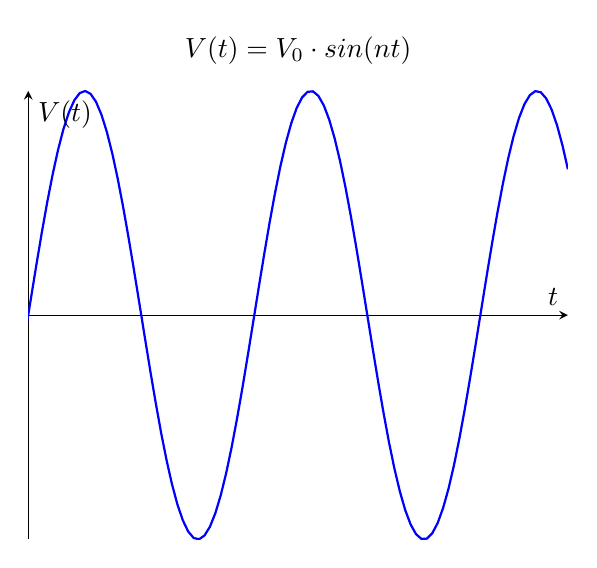
\begin{tikzpicture}
  \begin{axis}[ 
    xlabel=$t$,
    ylabel={$V(t)$},
    axis lines=middle,
    xtick=\empty,
	ytick=\empty,
	xmin=0,
	title={$V(t)=V_0\cdot sin(nt)$}
  ] 
    \addplot[blue,thick,samples=200] {5*sin(deg(3*x))}; 
  \end{axis}
\end{tikzpicture}
\hskip 10pt
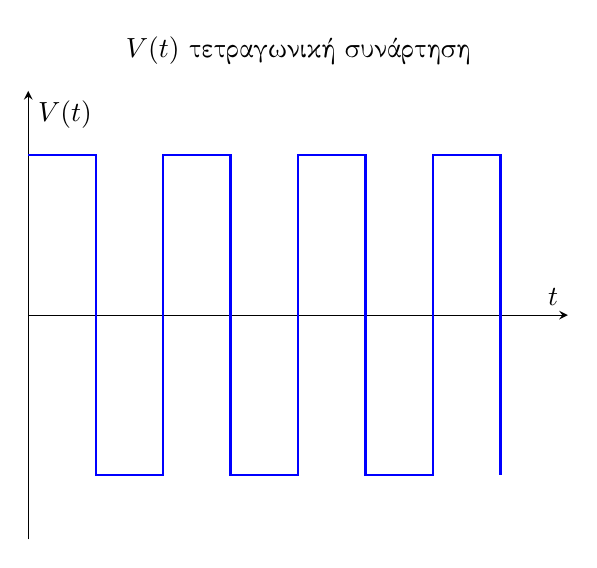
\begin{tikzpicture}
  \begin{axis}[ 
    xlabel=$t$,
    ylabel={$V(t)$},
    axis lines=middle,
    xtick=\empty,
	ytick=\empty,
	xmin=0,
	xmax=8,
	ymin=-1.4,
	ymax=1.4,
	title={$V(t)\text{ τετραγωνική συνάρτηση}$}
  ] 
    \addplot+[blue,thick,mark=none,const plot]
coordinates
{(0,1) (1,-1) (2,1) (3,-1) (4,1) (5,-1) (6,1) (7,-1)};
  \end{axis}
\end{tikzpicture}

\subsubsection{\(V(t) = V_0\)}
\[
\frac{\dif x}{\dif t}+ax=b
\]
Θα εξετάσω τη γενική λύση \(x_0(t)\) της ομογενούς ΔΕ, και \\
θα ψάξω μία ειδική λύση της μη ομογενούς ΔΕ.

Ομογενής: \(b=0 \implies \frac{\dif x}{\dif t} = -ax \implies x(t)=ce^{-at}.\)\\\(x(0)=0\implies c=0 \implies x_0(t)=0\).

Μη ομογενής: \(\frac{\dif x}{\dif t}+ax=b\).
\[
x(t)=k \implies \frac{\dif x}{\dif t}+ak=b \implies k =\frac{b}{a} \implies x(t)=k=\frac{b}{a}
\]

\begin{theorem*}{}
%\paragraph{Θ.}
Η γενική λύση της μη ομογενούς είναι:
\[x(t) = x_h(t)+x_i(t) \]
\end{theorem*}

Άρα \[
\begin{cases}
x(t) = ce^{-at} - \frac{b}{a} \\
x(0) = 0
\end{cases}
\implies 0=x(0)=c+\frac{b}{a}
\implies x(t) =\frac{b}{a}-\frac{b}{a}e^{-at} \text{ ή και }
 x(t) =\frac{b}{a}(1-e^{-at})
 \]

\begin{tikzpicture}
  \begin{axis}[ 
    xlabel=$t$,
    ylabel={$x(t)$},
    axis lines=left,
    xtick=\empty,
	ytick=\empty
  ] 
    \addplot[blue,thick,domain=0:5] {1-e^(-x)}; 
  \end{axis}
\end{tikzpicture}

 
\[
a=\frac{1}{RC}, \quad b= \frac{V_0}{R}
\]

\subsubsection{\(V(t)=V_0 \sin(nt)\)}
\[
\frac{\dif x}{\dif t} + ax = b\sin (nt)
\]

Είναι \(x_h(t) = ce^{-at}\).

Υποθέτω \(x(t) = c_2 \sin (nt) + c_3 \cos (nt) \). Τότε \( \frac{\dif x}{\dif t} = nc_2 \cos (nt) - nc_3 \sin (nt) \):

\[ \frac{\dif x}{\dif t} +ax =
\left( ac_2 - nc_3
\right)
\sin (nt) +
\left( ac_3 + nc_2
\right) \cos (nt)
= b \sin (nt) \implies
\]

\[
\implies
\begin{cases}
ac_2-nc_3&=b \\
nc_2+ac_3&=0 
\end{cases}
\implies \cdots \implies
\begin{cases}
c_2 &= \frac{ab}{a^2+n^2} \\
c_3 &= -\frac{bn}{a^2+n^2} 
\end{cases}
\]

Θυμάμαι ότι \(x(t) = x_h(t)+x_i(t) = c_1e^{-at} + \frac{ab}{a^2+n^2} \sin (nt) -  \frac{bn}{a^2+n^2} \cos (nt)\) και από το \(x(0)=0\) βρίσκω \(c_1 = \frac{bn}{a^2+n^2}\).

Άρα:
\[
x(t) = \frac{bn}{a^2+n^2} + \frac{ab}{a^2+n^2} \sin (nt) -  \frac{bn}{a^2+n^2} \cos (nt)
\]

Για το \(RC\) κύκλωμα, \(a=\frac{1}{RC} \leftarrow \) χρονική σταθερά κυκλώματος, \(b=\frac{V_0}{R}\), άρα:
\[
Q(t) = \frac{V_0C^2Rn}{C^2R^2n^2+1}e^{-\frac{t}{RC}} + \frac{CV_0\sin (nt) - C^2RnV_0 \cos (nt)}{C^2R^2n^2+1}
\]

\begin{attnbox}{}
\begin{align*}
p \cos (\omega t) + q \sin (\omega t) = \\
\sqrt{p^2+q^2} \left( \frac{p}{\sqrt{p^2+q^2}} \cos \omega t+ \frac{q}{\sqrt{p^2+q^2}} \sin \omega t \right) = \\
\sqrt{p^2+q^2} \left ( \sin \phi \cos \omega + \cos \phi \sin \omega t \right) = \\
\sqrt{p^2+q^2} \sin ( \omega t + \phi ), \quad \phi = \arctan \frac{p}{q}
\end{align*}
\end{attnbox}

Παρατηρούμε ότι ο πυκνωτής φορτίζει περισσότερο αν είναι μικρότερη η συχνότητα του εναλλασσόμενου ρεύματος.

\pgfplotsset{width=0.8\textwidth}
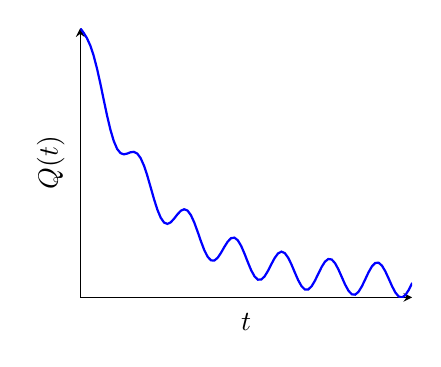
\begin{tikzpicture}
  \begin{axis}[ 
  	height=5cm,
    xlabel=$t$,
    ylabel={$Q(t)$},
    axis lines=left,
    xtick=\empty,
	ytick=\empty
  ] 
    \addplot[blue,samples=100,thick,domain=0:2*pi] {1.5*e^(-0.75*x)+0.1*sin(400*x)}; 
  \end{axis}
\end{tikzpicture}

\subsubsection{\(V(t) = \mathrm{square}(t)\)}
%\begin{tikzpicture}[domain=0:14]
%\draw (0,0) -- (0,4);
%\draw (0,4) -- (2,4);
%\draw (2,4) -- (2,0) node[anchor=west] {\(\pi\)};
%\draw (2,0) -- (2,-4) -- (4,-4) -- (4,4) -- (6,4) -- (6,-4);

%\draw[color=blue]
%plot (\x,{exp(-\x) + 0.35*sin(5*\x r)})
%node[right] {$f(x) = \sin x$};
%\end{tikzpicture}
\[
V(t)= \sum _{n = (1,3,5,\dots)} \frac{4}{n \pi} \sin (n t) =
\frac{4}{ \pi} \sin (n t) + \frac{4}{3 \pi} \sin (3 t) +
+ \frac{4}{5 \pi} \sin (5 t) \frac{4}{7 \pi} \sin (7 t) + \cdots
\]

Έτσι γίνεται η ανάλυση \textlatin{Fourier}, και αυτό θα το δούμε την επόμενη Τετάρτη, που θα πάμε στο Κεφάλαιο 8, που λέει σειρές \textlatin{Fourier}.

\[
V_N(t) = \sum _{n = (1,3,5,\dots)}^N \frac{4}{n \pi} \sin (n t)
\]
\[
V(t) = \sum _{n = (1,3,5,\dots)}^\infty \frac{4}{n \pi} \sin (n t) = \lim_{t \to \infty} V_N(t)
\]

\paragraph{}
Άρα:
\[
 \frac{\dif R}{\dif t}  + \frac{1}{RC}Q(t) = \frac{V_0 \sin (nt)}{R} \implies
 Q_n(t) = \frac{V_0C^2Rn}{C^2R^2n^2+1}e^{\frac{t}{RC}} + \frac{CV_0\sin (nt) - C^2RnV_0 \cos (nt)}{C^2R^2n^2+1}
\]

Οπότε αν:
\[
 \frac{\dif R}{\dif t}  + \frac{1}{RC}Q(t) = \frac{4}{\pi} \frac{\sin (nt)}{R} \implies
 Q_1(t) = \frac{4}{\pi} \left( \frac{C^2R}{C^2R^1+1} e^{-\frac{1}{RC}}+ \cdots \right)
\]
\[
 \frac{\dif R}{\dif t}  + \frac{1}{RC}Q(t) = \frac{4}{3\pi} \frac{\sin (3t)}{R} \implies
 Q_3(t) = \frac{4}{3\pi} \left( \frac{3C^2R}{9C^2R^1+1} e^{-\frac{1}{RC}}+ \cdots \right)
\]
\[
 \frac{\dif R}{\dif t}  + \frac{1}{RC}Q(t) = \frac{4}{5\pi} \frac{\sin (5t)}{R} \implies
 Q_5(t) = \cdots
\]

Άρα:
\[
Q(t) = \sum_{n \in \lbrace1,3,5,\dots\rbrace}Q_n(t)
\]

Γιατί όμως, αν \(V_1(t) \rightarrow Q_1(t), \ V_2(t) \rightarrow Q_2(t)\), τότε \(k_1V_1+k_2V_2 = k_1Q_1 +k_2Q_2\) σε αυτό το κύκλωμα (αρχή επαλληλίας/γραμμικότητα)?


\section{Κεφάλαιο 8: Σειρές Fourier}

\begin{defn*}{}
Μία συνάρτηση \(f(t)\) λέγεται \textbf{τμηματικά συνεχής} στο \([t_1,t_2]\) ανν μπορώ να διαμερίσω:
\[ [t_1,t_2] = [\tau_0,\tau_1] \cup [\tau_1,\tau_2] \cup \cdots \cup [\tau_{n-1},\tau_n] \]
όπου \(\tau_0 = t_1,\ \tau_n = t_2\), τέτοια ώστε \(f(t)\) συνεχής στο κάθε \((\tau_{i-1},\tau_i)\), και υπάρχουν \(\lim_{t \to \tau_i^-} f(t),\ \lim_{t \to \tau_1^+}\ f(t) \forall i\)
\end{defn*}

\textit{π.χ}

%TODO Graph1
Η \(f(t)\) είναι τμηματικά συνεχής στο \([-\pi,3\pi]\), επειδή, για \(t_1=-\pi,t_2=3\pi\):
\[
[-\pi,3\pi] = [-\pi,0] \cup [0,\pi] \cup [\pi,2\pi] \cup [2\pi,3\pi]
\]
Στα \( (-\pi,0),\ (0,\pi) ,\   (\pi,2\pi) ,\   (2\pi,3\pi)\) η \(f\) είναι συνεχής, και υπάρχουν τα αντίστοιχα πλευρικά όρια, %TODO
άρα η \(f\) είναι τμηματικά συνεχής.

\subsubsection{Συνθήκες του \textlatin{Dirichlet}}
\begin{enumerate}
\item Η \(f(t)\) είναι ορισμένη στο \((-L,L)\)
\item Η \(f(t)\) είναι τμηματικά συνεχής στο \((-L,L)\)
\item Η \(f(t)\) είναι περιοδική με περίοδο \(2L\).
\end{enumerate}

\subsection*{}

\begin{theorem*}{}
Έστω \(f(t)\) η οποία ικανοποιεί τις συνθήκες \textlatin{Dirichlet} στο \((-L,L)\). Τότε:
\begin{enumerate}
\item
Για κάθε σημείο συνέχειας της \(f(t)\):
\[
f(t) = \frac{a_0}{2}+\sum_{n=1}^\infty a_n \cos \frac{n\pi t}{L}
+\sum_{n=1}^\infty b_n \sin \frac{n\pi t}{L}
\]
όπου:
\begin{align*}
a_n&=\frac{1}{L} \int_{-L}^L f(t) \cos \frac{n\pi t}{L} \dif t \\
b_n&=\frac{1}{L} \int_{-L}^L f(t) \sin \frac{n\pi t}{L} \dif t
\end{align*}

\item Σε κάθε σημείο ασυνέχειας \(\tau\):
\[
\frac{1}{2} \left( \lim_{t \to \tau^-}f(t) + \lim_{t \to \tau^+}f(t) \right) 
= \frac{a_0}{2}+\sum_{n=1}^\infty a_n \cos \frac{n\pi t}{L}
+\sum_{n=1}^\infty b_n \sin \frac{n\pi t}{L}
\]
\end{enumerate}

\end{theorem*}

\paragraph{Παρ.}
\(f(t) = \text{τετραγωνικός παλμός}\)

\subparagraph{Λύση}
Η \(f(t)\) ικανοποιεί τις Σ.\textlatin{D} με \(L=\pi\)
\begin{align*}
a_0 &= \frac{1}{\pi} \int_{-\pi}^\pi f(t) \dif t = \frac{1}{\pi}\int_{-\pi}^0(-1)\dif t+\frac{1}{\pi}\int_{-\pi}^0 1\dif t = -1 + 1 = 0 \\
b_n &= \frac{1}{\pi} \int_{-\pi}^\pi f(t) \sin \frac{n \pi t}{\pi} \dif t
= \frac{2}{\pi} \int_0^\pi 1 \sin (nt) \dif t \\
&= \frac{2}{\pi} \cdot \left( \frac{-\cos nt}{n} \right)_{t=0}^\pi
=\frac{2}{\pi} \cdot \left( \frac{1-\cos n\pi}{\pi} \right) =
\frac{2}{\pi} \left( \frac{1-(-1)^n}{n} \right) = \frac{2}{n\pi} \text{ για άρτια }n
\end{align*}

Άρα:
\begin{align*}
a_0=a_1=a_2=\cdots=0 \\
b_1=\frac{4}{\pi}, \quad b_3=\frac{4}{3\pi} \\
\quad b_2=0, \quad b_4 = 0, \dots
\end{align*}
%a_n &= \frac{1}{\pi} \int_{-\pi)^\pi \underbrace{f(t)}_{\text{άρτια}} \underbrace{\cos \frac{n \pi t}{\pi}}_{\text{άρτια}}

\paragraph{Απόδειξη} (Μερική)

Θα δεχτούμε ότι η \(f(t)\) γράφεται στη μορφή \(f(t) = \frac{a_0}{2}+\sum_{n=1}^\infty a_n \cos \frac{n\pi t}{L}
+\sum_{n=1}^\infty b_n \sin \frac{n\pi t}{L}\),
και θα δείξουμε τους τύπους \(
a_n=\frac{1}{L} \int_{-L}^L f(t) \cos \frac{n\pi t}{L} \dif t ,\ 
b_n=\frac{1}{L} \int_{-L}^L f(t) \sin \frac{n\pi t}{L} \dif t
\)

Έστω \(f(t)= \frac{a_0}{2}+\sum_{n=1}^\infty a_n \cos \frac{n\pi t}{L}
+\sum_{n=1}^\infty b_n \sin \frac{n\pi t}{L}\).
Tότε: \[\int_{-L}^L f(t) \dif t = \int_{-L}^L f(t) \cdots t
= \int_{-L}^L \frac{a_0}{2} \dif t +
 \int_{-L}^L a_1 \cos \frac{\pi t}{L} \dif t +
 \int_{-L}^L a_2 \cos \frac{2\pi t}{L} + \cdots  = a_0\cdot L + 0 + 0 + \dots
\]
Άρα:
\[
a_0 = \frac{1}{L} \int_{-L}^L f(t) \dif t
\]

\subparagraph{Συνέχεια αόδειξης}
Υποθέτω ότι υπάρχει \textbf{κάποια} σειρά της μορφής *, θα δείξω ότι οι συντελεστές δίνονται από τους τύπους **.
ίό
Παρνω τυχόν \(m \in \mathbb N\) και εξετάζω το
\begin{align*}
\int_{-L}^L f(t) \cos \frac{m\pi t}{L} \dif t
&= \\ &=
\int_{-L}^L \left( \frac{a_0}{2}+\sum_{n=1}^\infty a_n \cos \frac{n\pi t}{L}
+\sum_{n=1}^\infty b_n \sin \frac{n\pi t}{L}\right)\cos \frac{m\pi t}{L} \dif t
\\ &=
\underbrace{\int_{-L}^L \frac{a_0}{2}\cos \frac{m\pi t}{L} \dif t}_{
=0\text{ ολοκληρώνω πάνω σε }m\text{ περιόδους}
}
+ \sum_{n=1}^\infty \int_{-L}^L a_n \cos \frac{n\pi t}{L} 
\cos \frac{m \pi t}{L} \dif t
+ \underbrace{\sum_{n=1}^\infty \int_{-L}^L b_n \sin \frac{n\pi t}{L} 
\cos \frac{m \pi t}{L} \dif t}_{
=\frac{b_n}{2} \left( \int_{-L}^L\sin\frac{n\pi t + m\pi t}{L} \dif t +
\int_{-L}^L\sin\frac{n\pi t - m\pi t}{L} \dif t
\right) = 0
}
\\ &=
 \sum_{n=1}^\infty a_n \int_{-L}^L \cos\frac{n\pi t}{L} \cos\frac{m\pi t}{L } \dif t
\\ & \overset{\cos a \cdot \cos \beta= \frac{cos(a+\beta)+cos(a-\beta}{2}}{=} 
 \sum_{n=1}^\infty \frac{a_n}{2} \int_{-L}^L \left( \cos \frac{(n+m)\pi t}{L}
+ \cos \frac{(n-m)\pi t}{L}
\right) \dif t
\\ &=
 \sum_{n=1}^\infty \begin{cases}
0, \quad & n \neq m \\
a_nL, & n=m
\end{cases} \\
&= a_mL
\end{align*}

Επομένως:
\[
a_m = \frac{1}{L} \int_{-L}^L f(t) \cos \frac{n\pi t}{L} \dif  t
\]

Αντιστοίχως αποδεικνύεται και η σχέση για το \(b_m\).

Να σημειωθεί ότι οι συνθήκες του \textlatin{Dirichlet} είναι ικανές, αλλά όχι αναγκαίες.

\subsubsection{}
\begin{gather*}
f(t) = 
\sum_{-\infty}^\infty c_ne^{\frac{in\pi t}{L}} \\
c_n = \frac{1}{2L} \int_{-L}^L e^{-in\pi t}{L} \dif t
\end{gather*}

\paragraph{Απόδειξη}
\begin{align*}
f(t) = \frac{a_0}{2}+\sum_{n=1}^\infty a_n \cos \frac{n\pi t}{L}
+\sum_{n=1}^\infty b_n \sin \frac{n\pi t}{L} &=
\frac{a_0}{2} +
%\sum_{n=1)^\infty a_n \frac{e^{\frac{in\pi t}{L}}+e^{\frac{-in\pi t}{L}}}{2}
%+\sum_{n=1)^\infty b_n \frac{e^{\frac{in\pi t}{L}}-e^{\frac{-in\pi t}{L}}}{2i}
\\ &=
%\begin{align*}
\frac{a_0}{2}
+ \sum_{n=1}^\infty \cdots e^{\frac{in\pi t}{L}}
+ \sum_{n=1}^\infty \frac{a_n-ib_n}{2}
e^{\frac{in\pi t}{L}} +
+ \sum_{n=-1}^{-\infty} \frac{a_{-n}+ib_{-n}}{2}
e^{\frac{in\pi t}{L}}
\end{align*}

Άρα \[
f(t) = \sum_{n=-\infty}^\infty c_n e^{\frac{in\pi t}{L}}
\]

όπου: \[
c_n = \begin{cases}
\frac{a_n-ib_n}{2},\quad & n \in \mathbb Z^+ \\
\frac{a_{-n}+ib_{-n}}{2},\quad & n \in \mathbb Z^- \\
\frac{a_0+ib_0}{2},\quad & n=0
\end{cases}
\]

Αφήνεται ως άσκηση για τον αναγνώστη να αποδειχθεί ότι:
\[
c_n =
\frac{1}{2L}
\int_{-L}^L f(t) e^{\frac{-in\pi t}{L}} \dif t
\]

\subsection{Παράδειγμα}
\begin{center}
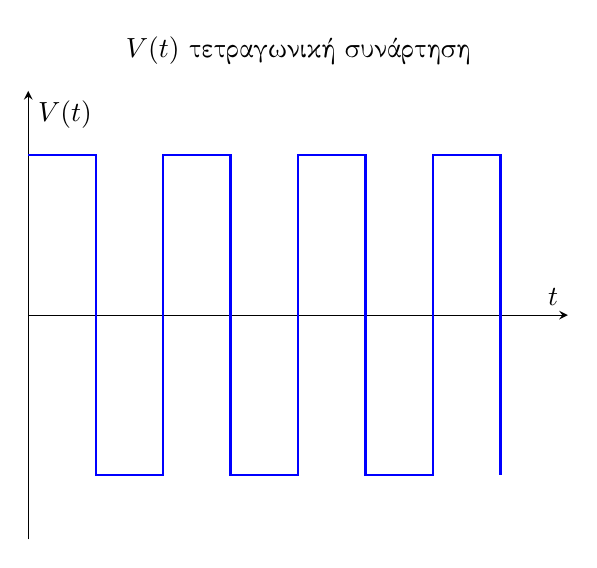
\begin{tikzpicture}
%TODO L = \pi, A = 1
  \begin{axis}[ 
    xlabel=$t$,
    ylabel={$V(t)$},
    axis lines=middle,
    xtick=\empty,
	ytick=\empty,
	xmin=0,
	xmax=8,
	ymin=-1.4,
	ymax=1.4,
	title={$V(t)\text{ τετραγωνική συνάρτηση}$}
  ] 
    \addplot+[blue,thick,mark=none,const plot]
coordinates
{(0,1) (1,-1) (2,1) (3,-1) (4,1) (5,-1) (6,1) (7,-1)};
  \end{axis}
\end{tikzpicture}
\end{center}

Θα βρω την \textbf{εκθετική} σειρά της \(f(t)\).

\begin{align*}
c_n &= \frac{1}{2\pi}
\int_{-\pi}^\pi f(t)e^{-int}\dif t \\
&=
\frac{1}{2\pi}
\int_{-\pi}^0(-1)\cdot e^{-int} \dif t
+
\int_{0}^0(\pi)1\cdot e^{-int} \dif t
\\ &=
\frac{1}{2\pi}
\left(
- \int_{-\pi}^0e^{-int}\dif t
+ \int_0^\pi e^{-int} \dif t
\right)
\\ &=
\frac{1}{2\pi}
\left(
 \left. \frac{e^{-int}}{in} \right|_{-\pi}^0
+ \left. \frac{e^{-int}}{in} \right|_0^\pi
\right)
\\ &=
\frac{1}{2\pi} \left(
\frac{1}{in} - \frac{e^{-in\pi}}{in} - \frac{e^{-in\pi}}{in} + \frac{1}{in}
\right)
\\ &=
\frac{1}{2\pi}
\left(
\frac{2}{in}
- \frac{2\cos (n \pi)}{in}
\right)
\\ c_n &=
\frac{i}{n\pi}
\cdot \big(
1-\cos n\pi
\big)
\end{align*}

\[
\begin{array}{r|l}
n & c_n \\
-2 & 0 \\
-1 & \frac{2i}{\pi} \\
0 & 0 \\
1 & \frac{-2}{\pi} \\
2 & 0 \\
3 & \frac{-2i}{3\pi}
\end{array}
\]

Άρα:

\[
f(t) = \cdots + \frac{2i}{3\pi} e^{i3t} + \frac{2i}{\pi} e^{-it}
- \frac{2i}{\pi} e^{it}
- \frac{2i}{3\pi} e^{i3t} + \cdots
\]

Ερωτήματα για τον αναγνώστη:
\begin{enumerate}
\item
Πότε έχει η τριγωνομετρική σειρά μόνο ημίτονα/μόνο συνημίτονα?
\item
Πότε έχει η εκθετική σειρά μόνο πραγματικούς/μόνο εκθετικούς όρους?
\end{enumerate}

\subsection{}
\begin{defn*}{}
Συμβολίζω με \(\mathfrak{F}_L\) το σύνολο των συναρτήσεων που ικανοποιούν τις συνθήκες \textlatin{Dirichlet} (με ημιπερίοδο \(L\))
\end{defn*}

\begin{theorem*}{}
Το \(\mathfrak F_L\) είναι διανυσματικός χώρος. 
\end{theorem*}
\paragraph{Απόδειξη}

Έστω \(f,g \in \mathfrak F_L\) και \(\kappa,\lambda \in \mathbb C\). Θα δείξω ότι \(\kappa f + \lambda g \in \mathfrak F_L\).

\subparagraph{Πράγματι}
\begin{enumerate}
\item
Αν οι \(f,g\) είναι ορισμένες στο \([-L,L]\) τότε και η \(\kappa f + \lambda g\) είναι ορισμένη στο \([-L,L]\).
\item
\begin{align*}
(\kappa f + \lambda g)(t+2L) &= \kappa f (t+2L) + \lambda g (t+2L) \\
&= \kappa f(t) + \lambda g(t) \\
&= (\kappa f + \lambda g)(t)
\end{align*}
Άρα η \(\kappa f + \lambda g\) έχει περίοδο \(2L\).

\item
Αν η \(f\) και η \(g\) είναι τμ. συνεχείς στο \([-1,1]\), τότε και η \(\kappa f+\lambda g\) είναι τμ. συνεχείς.
\end{enumerate}

Από τα 1,2,3, η \(\kappa f + \lambda g \in \mathfrak F_L\).

\begin{theorem*}{}
Το σύνολο \(  \left\lbrace e^{\frac{in\pi t}{L}} \right\rbrace^\infty_{-\infty} \) είναι μια ορθογώνια βάση του \(\mathfrak F_L\).
\tcblower
\paragraph{Δηλαδή}
κάθε \(f(t) \in \mathfrak{F}_L\) μπορεί να γραφεί:
\[
f(t) =
\sum_{n=-\infty}^\infty c_n e^{\frac{in\pi t}{L}}
\]

Επιπλέον \(\forall n,m,\ m \neq n\ e^{\frac{in\pi t}{L}} \perp e^{\frac{im\pi t}{L}}\)

Δηλαδή:
\[
e^{\frac{im\pi t}{L}} \cdot
e^{\frac{in\pi t}{L}} = 0
\]

Δηλαδή:
\[
\int_{-L}^L e^{\frac{im\pi t}{L}} \cdot
 e^{\frac{in\pi t}{L}} \dif t =0
\]

Για να ορίσω το εσωτερικό γινόμενο, θέλω \(
\|\vec{x}\|^2 = \vec{x} \cdot \vec{x} = \sum_n x_n\bar{x_n} = \sum(x_n)^2
\)

\[
f \cdot g = \int_{-L}^L f(t) \overline{g(t)} \dif t
\]

Άρα
\[
e^{\frac{im\pi t}{L}} \cdot
e^{\frac{in\pi t}{L}} =
\int_{-L}^L e^{\frac{im\pi t}{L}} e^{\frac{in\pi t}{L}} \dif t =
\int_{-L}^L e^{\frac{i(m-n)\pi t}{L}} \dif t =
\begin{cases}
2L, \quad & m=n \\
0, \quad & m \neq n
\end{cases}
\]

\end{theorem*}

\begin{itemize}
\item \(\mathfrak F_L\) το σύνολο των συναρτήσεων που ικανοποιούν \textlatin{Dirichlet}
\item Το \(\mathfrak F_L\) είναι ΔΧ
\item Το \(  \left\lbrace e^{\frac{in\pi t}{L}} \right\rbrace_{n \mathbb Z}\) είναι μια ορθογώνια βάση του \(\mathfrak{F_L}\)
\item Το \(  \left\lbrace \cos{\frac{in\pi t}{L}} \right\rbrace_{n =0}^{\infty} \cup \left\lbrace \sin{\frac{in\pi t}{L}} \right\rbrace_{n =1}^\infty\) είναι μια ορθογώνια βάση του \(\mathfrak{F_L}\)
\item \(\underbrace{f(t)}_{\mathclap{\text{περιοδική, με ημιπερίοδο $L$}}} = \sum_{n=-\infty^\infty} c_n e^\frac{in\pi t}{L}\), με
\[
c_n = \frac{1}{2L} \int_{-L}^L f(t)e^\frac{in\pi t}{L} \dif t
\]
\end{itemize}

%TODO Kehagias 01 Graph
\begin{align*}
\vec{x} = [x_1 x_2 x_3] &= x_1 \vec{e_1} +x_2 \vec{e_2}+x_3 \vec{e_3}
\\ &=
\mathrm{Proj}(\vec{x}, \vec{e_1})
+\mathrm{Proj}(\vec{x}, \vec{e_2})
+ \mathrm{Proj}(\vec{x}, \vec{e_3})
\\ &=
\sum_{n=1}^3
\vec{x} \cdot \vec{e_n} \cdot \frac{\vec{e_n}}{\norm{\vec{e_n}}}
\end{align*}

Άρα:
\[
f(t) = \sum_{n=-\infty^\infty} c_n e^\frac{in\pi t}{L}
= \sum_{n=-\infty^\infty} \mathrm{Proj} \left( f(t), e^\frac{in\pi t}{L} \right)
\]
όπου \(\mathrm{Proj} \left( f(t), e^\frac{in\pi t}{L} \right) =
f(t)\bullet e^\frac{in\pi t}{L} \frac{e^\frac{in\pi t}{L}}{\norm{e^\frac{in\pi t}{L}}}
\)

\begin{align*}
f(t) \bullet e^\frac{in\pi t}{L} &= \int_{-L}^L f(t) \cdot \overline{e^\frac{in\pi t}{L}} \dif t 
\\
\norm{e^\frac{in\pi t}{L}} &= \int_{-L}^L e^\frac{in\pi t}{L} \cdot e^\frac{-in\pi t}{L} \dif t = 2L
\end{align*}

\begin{theorem}{\textlatin{Plancherel}}{}
\[
\frac{1}{2L} \int_{-L}^L f(t) \overline{g(t)} \dif t =
\sum_n c_n \overline{r_n}
\]

Η \(\begin{cases}
f(t)&= \sum_n c_n e^\frac{in\pi t}{L} \\
f(t)&= \sum_n r_n e^\frac{in\pi t}{L}
\end{cases}\)
\end{theorem}

\paragraph{Απόδειξη}
\begin{align*}
\frac{1}{2L} \int_{-L}^L f(t) \overline{g(t)} \dif t &=
\frac{1}{2L} \int_{-L}^L 
	\left( \sum_{n=-\infty}^\infty c_n e^\frac{in\pi t}{L}
	\right)
	\overline{\left(
	\sum_{m=-\infty}^\infty c_m e^\frac{im\pi t}{L}
	\right)}
	\dif t
\\ &=
\frac{1}{2L} \int_{-L}^L \left(
\sum_{n=-\infty}^\infty \sum_{m=-\infty}^\infty
c_n e^\frac{in\pi t}{L}
\overline{r_m} e^\frac{im\pi t}{L} \right) \dif t
\\ &=
\frac{1}{2L}
\sum_{n=-\infty}^\infty
\sum_{m=-\infty}^\infty
c_n \bar{r_m}
\underbrace{\int_{-L}^L
e^\frac{i(n-m)\pi t}{L} \dif t}_{
\begin{cases}
0 \qquad & m \neq n\\
2L & m = n
\end{cases}
}
\\ &= \frac{1}{2L} 2L \sum_n c_n\bar{r_n}
\end{align*}

Γενικά:
\[
f(t) \leftrightarrow \vec{c} = [ \dots \ c_{-1}\  c_0\  c_1\ c_2\ \dots ]
\]
(με την επιφύλαξη ότι σε πεπερασμένο αριθμό σημείων μπορεί να αλλάζει η τιμή της συνάρτησης)

Σύμφωνα με το θεώρημα:
\begin{align*}
f(t) &\leftrightarrow \vec{c} \\
g(t) &\leftrightarrow \vec{r} \\
 \frac{1}{2L} f\bullet g &= \vec{c} \bullet \vec{r}
\end{align*}

\begin{theorem}{Πόρισμα (\textlatin{Parseval})}{}
\[
\frac{1}{2L} \int_{-L}^L
\left|
f(t)
\right|^2 \dif t
= \sum_n
|c_n|^2
\]
%TODO Graph 02 Kehagias
\end{theorem}

\begin{theorem}{}{}
Αν \(f(t) \in \mathfrak F_L\) και \(f(t) = \sum_n c_n e^\frac{in\pi t}{L}\), τότε:
\begin{align*}
\od{f}{t}&=\sum_n c_n \frac{in\pi}{L} e^\frac{in\pi t}{L} \\
\int f(t)&=\sum_n c_n \frac{L}{in\pi} e^\frac{in\pi t}{L}
\end{align*}

Τα ίδια για ημίτονα και συνημίτονα
\end{theorem}

\paragraph{Παράδειγμα}
Δίνεται η \(f(t)
= \begin{cases}
|t| &\qquad t \in [-\pi,\pi] \\
\text{περιοδική επέκταση} &\qquad t \notin [-\pi,\pi]
\end{cases}
\)
Να βρεθεί η Σειρά (\textlatin{Fourier}) της \(f(t)\).
\subparagraph{Λύση}
%TODO Kehagias Graph 03
Αφού λοιπόν \(g(t)=
\frac{4}{\pi} \cdot
\left(
\sin t + \frac{\sin(3t)}{3} + \frac{\sin(5t)}{5} + \dots
\right)
\), τότε:
\begin{align*}
f(t) &=
c - \frac{4}{\pi}
\left(
\cos t + \frac{\cos 3t}{3^2}
+ \frac{\cos 5t}{5^2}
\right)
\\ f\left(\frac{\pi}{2}\right) &= \frac{\pi}{2} = c
\end{align*}

Άρα τελικά:
\[
f(t) = \frac{\pi}{2} - \frac{4}{\pi}
\left(
\cos t + \frac{\cos 3t}{3^2}
+ \frac{\cos 5t}{5^2}
\right)
\]

Παρατηρώ ότι η \(f\) έχει ασθενέστερες υψηλές συχνότητες από τη \(g\).

\paragraph{Παράδειγμα}
Να υπολογιστεί το:
\[
S_1 = 1 - \frac{1}{3} + \frac{1}{5} - \frac{1}{7} + \frac{1}{9} + \cdots
\]

Είναι \begin{align*}
g\left( \frac{\pi}{2}\right) &=
\frac{4}{\pi}\left(
\sin \frac{\pi}{2}+\frac{\sin\frac{3\pi}{2}}{3}
+ \frac{\sin\frac{5\pi}{2}}{5}
\right)
\\ 
1 = g\left( \frac{\pi}{2}\right) &= \frac{4}{\pi}
\left(
1-\frac{1}{3}+\frac{1}{5}-\cdots
\right) = S_1
\end{align*}

\paragraph{Παράδειγμα}
Να υπολογιστεί το:
\[
S_1 = 1 + \frac{1}{3^2} + \frac{1}{5^2} + \frac{1}{7^2} + \cdots
\]
\subparagraph{Λύση}
\begin{align*}
0=f(0)&=\frac{\pi}{2} - \frac{4}{\pi} \cdot\left(
1+\frac{1}{3^2}+\frac{1}{5^2}+\cdots
\right)
\\ \frac{\pi^2}{8} &= 1 + \frac{1}{3^2} + \frac{1}{5^2} + \cdots
\end{align*}




\section{Κεφάλαιο 9: Μετασχηματισμός Fourier}
%TODO Kehagias Graph 04
\begin{theorem*}{}
Έστω ότι η \(f(t)\) ικανοποιεί τα εξής:
\begin{enumerate}
\item Τις συνθήκες \textlatin{Dirichlet} \(\forall L \in  \mathbb R \)
\item \( \int_{-\infty}^\infty |f(t)| \dif t < \infty\) (δηλ. η \(f(t)\) είναι απολύτως ολοκληρώσιμη)
\end{enumerate}

Τότε:
\[
f(t) = \frac{1}{2\pi}
\int_{-\infty}^\infty F(\omega) e^{i\omega t} \dif t
\]
όπου:
\[
F(\omega) = \int_{-\infty}^\infty f(t)e^{-i\omega t} \dif t
\]

\end{theorem*}

\paragraph{Απόδειξη}
Δίνεται η \(f(t)\). Διαλέγω τυχόν \(t\) και ορίζω την \(f_T(t) = f(t)\quad \forall t \in \left[ -\frac{T}{2}, \frac{T}{2} \right]\), που έχει σειρά \textlatin{Fourier}:
\[
f_T(t) = \sum_{n=-\infty}^\infty c(n) e^\frac{in2\pi t}{T}
\]
όπου
\[
c(n) = \frac{1}{T} \int_{-\frac{T}{2}}^\frac{T}{2} f(t) e^{-\frac{in2\pi t}{T}} \dif t
\]

Θέτω \(\delta \omega = \frac{2\pi}{T},\ \omega = n\cdot \delta \omega = \frac{2n\pi}{T}
\)

\begin{align*}
f_T(t) &= \sum_{n=-\infty}^\infty
\left(
\frac{1}{T} \int_{-\frac{T}{2}}^\frac{T}{2} f(t) e^{-\frac{in2\pi t}{T}} \dif t
\right) e^\frac{in2\pi t}{T}
\\ &= \frac{1}{2\pi}
\sum_{n=-\infty}^\infty
\left(
\frac{2\pi}{T}
\int_{-\frac{T}{2}}^\frac{T}{2}
f_T(t)e^{-i\omega t} \dif t
\right) e^\frac{in2\pi t}{T}
\\ &=
\frac{1}{2\pi}
\sum_{n=-\infty}^\infty
\left(
\int_{-\frac{T}{2}}^\frac{T}{2}
f_T(t)e^{-i\omega t} \dif t
\right)
e^{i\omega t} \delta \omega
\\ &=
\frac{1}{2\pi}
\int_{-\infty}^\infty
\underbrace{\left(
\int_{-\infty}^\infty
f(t)e^{i\omega t} \dif t
\right)}^{F(\omega)}
e^{i\omega t}
\dif \omega
\end{align*}

Την \(F(\omega)\) την ονομάζουμε \textbf{\textlatin{Fourier} μετασχηματισμένη} της \(f(t)\), και γράφουμε:
\[
\mathscr{F}\bigg( f(t) \bigg) = F(\omega)
\]

\begin{tcolorbox}
\[
F(\omega) = \mathscr{F} f(t)
\quad
f(t) = \mathscr{F}^{-1} \left( F(\omega) \right)
\]
\end{tcolorbox}

\paragraph{Παρ.}
\[
f(t)=
\begin{cases}
1 \quad |t|<a\\
0 \quad |t|\geq a
\end{cases}
\]

\begin{align*}
F(\omega) = \int_{-\infty}^\infty f(t)e^{-i\omega t} \dif t
&= \int_{-a}^a 1 e^{-i \omega t} \dif t = -\frac{1}{i \omega } e^{-i \omega t} \dif t
\\
&=
\frac{2}{\omega}
\left(
\frac{-e^{-i \omega a}}{2i}
\right)
\\ &= 2 \frac{\sin( \omega a)}{\omega}
\end{align*}

\paragraph{Παρ.}
\[
f(t)=e^{-|t|}
\]

\begin{align*}
F( \omega )&=\int_{- \infty }^ \infty e^{-|t|} e^{-i \omega t} \dif t
\\ &=
\int_{- \infty }^0 e^t e^{-i \omega t} \dif t
+ \int_0^ \infty e^{-t}e^{-i \omega t} \dif t
\end{align*}

\begin{align*}
\int_0^ \infty e^{-t}e^{-i \omega t} \dif t &=
-\left. \frac{1}{1+i\omega} \right|_{t=0}^\infty
\\
&= -\frac{1}{1+i\omega} \left(
e^{-(1+i \omega )\cdot\infty}-e^{-(1+i \omega )\cdot0}
\right)
\\ &=
-\frac{1}{1+i\omega}
\Bigg(
0-1
\Bigg)
\\ &= \frac{1}{1+i\omega}
\end{align*}


Άρα:
\begin{align*}
\int_{- \infty }^0 e^t e^{-i \omega t} \dif t
+ \int_0^ \infty e^{-t}e^{-i \omega t} \dif t
&= \frac{1}{1-i \omega }+\frac{1}{1+i \omega }\\
&=
\boxed{
\frac{2}{1+\omega^2} = \mathscr{F} \left(
e^{-|t|}
\right)
}
\end{align*}

\begin{tcolorbox}
Ο Μ/Σ \textlatin{Fourier} εφαρμόζεται μόνο σε απόλυτα ολοκληρώσιμες \(f(t)\). Δηλαδή υποθέτω ότι \[
\int_{- \infty }^ \infty 
\left|
f(t)
\right|
\dif t = M <  \infty 
\]

Αυτό το κάνω, διότι \(\int_{- \infty }^ \infty |f(t)| \dif t < M < \infty\) είναι ικανή συνθήκη για να υπάρχει το \(\int_{- \infty }^ \infty f(t)e^{-i\omega t}\).

Έχει μία σημαντική συνέπεια:
\[
\lim_{t\to\pm\infty} f(t) = 0
\]

Για παράδειγμα, οι \(\mathscr{F}(e^t)\) και \(\mathscr{F}(e^{-t})\) δεν υπάρχουν, ενώ ο \(\mathscr{F}(e^{-|t|})\) υπάρχει διότι η \(e^{-|t|}\) είναι απόλυτα ολοκληρώσιμη.

Επίσης \( \int_{-\infty}^ \infty |F(\omega)| \dif \omega = M' < \infty \)
\end{tcolorbox}

\begin{theorem}{}{}
\[
\mathscr{F}(\kappa f + \lambda g) = \kappa \mathscr{F}(f)+\lambda \mathscr{F}(g)
\]
\tcblower
\paragraph{Παρ.}
\[
 \mathscr{F} (3\cdot \mathrm{square} + 5\cdot e^{-|t|}) = 6 \frac{\sin(\omega)}{\omega}+\frac{10}{1+\omega^2}
\]
\end{theorem}
Η απόδειξη είναι εύκολη και αφήνεται για τον αναγνώστη.

\begin{attnbox}{}
Το \textlatin{Wolfram} επιστρέφει τους Μ/Σ \textlatin{Fourier} με διαφορετικό παράγοντα, για λόγους συμμετρίας! (\(\frac{1}{\sqrt{2\pi}}\) έναντι \(\frac{1}{2\pi}\)). Στις σημειώσεις τηρείται η ιστορική σύμβαση που ακολουθείται και από προγράμματα όπως, π.χ. \textlatin{Matlab}.
\end{attnbox}

\begin{theorem}{}{}
Έστω \(F( \omega )= \mathscr{F} \left( f(t) \right)\), τότε:
\[
 \mathscr{F} \left( F(t) \right) = 2\pi f(-\omega)
\]

Δηλαδή:
\[
 \mathscr{F} \left(  \mathscr{F} \left( f(t) \right) \right) = 2\pi f(-t)
\]
\end{theorem}
\paragraph{Απόδ.}
\begin{align*}
 \mathscr{F} \left( f(t) \right) = F(\omega) = \int_{-\infty}^\infty f(t)e^{-i\omega t} \dif t \\
 \mathscr{F}^{-1} \left( F(\omega)) \right) = f(t) = \frac{1}{2\pi}\int_{-\infty}^\infty F(\omega)e^{i\omega t} \dif \omega \\
 2\pi f(-t) = \int_{-\infty}^ \infty F(\omega) e^{-i\omega t} \dif \omega
 \\
= \int_{-\infty}^ \infty F(\tau)e^{-i\tau w} \dif \tau = 2\pi f(-w) \\
=  \mathscr{F} \left( F(\tau) \right) =2\pi f(-w)
\end{align*}

\paragraph{Παρ.}
\[
 \mathscr{F} \left(
 \frac{1}{1+t^2}
 \right)
\]
\subparagraph{Λύση}
\[
\dots = \int_{-\infty}^\infty \dots
\]
ή

Παρατηρώ ότι \( \mathscr{F} (\frac{1}{2}e^{-|t|}) = \frac{1}{1+\omega^2} = F(\omega) = F(-\omega)\)

Άρα \(F(t) = \frac{1}{1+t^2}\)
\[
 \mathscr{F}  \left(
 \frac{1}{1+t^2}
 \right) =  \mathscr{F} \left( F(t) \right) = 2\pi f(-\omega) = \pi e^{-|\omega|}
\]

\begin{theorem}{}{}
\[
 \mathscr{F} \left( f(at) \right) = \frac{1}{a} F \left(\frac{\omega}{a} \right)
\]
\end{theorem}
\paragraph{Απόδ.}
\begin{align*}
 \mathscr{F} \left( f(at) \right)&=\int_{-\infty}^\infty f(at) e^{-i  \omega t} \dif t
 \\ &=
 \int_{-\infty}^\infty f(at)e^{-i\frac{\omega}{a}at} \dif t
 \\ &=
\frac{1}{a}  \int_{-\infty}^\infty f(at)e^{-i\frac{\omega}{a}at} \dif (at)
=
\frac{1}{a} \int_{-\infty}^\infty f(\kappa) e^{-i\frac{\omega}{a}\kappa} \dif \kappa
= \frac{1}{a}	F\left( \frac{\omega}{a}\right)
\end{align*}

\paragraph{Παρ.}
\[
 \mathscr{F} \left( \frac{1}{4+9t^2} \right)
 = \frac{1}{4} \mathscr{F} \left( \frac{1}{1+\frac{9}{4}t^2} \right) 
 = \frac{1}{4}  \mathscr{F} \left( \frac{1}{1+\left(\frac{3}{2}t\right)^2} \right)
\]

Για \(f(t) = \frac{1}{1+t^2}, \quad F(\omega) = \pi e^{-|\omega|}\),
\[
f(\frac{3}{2}t = \frac{1}{1+\frac{9}{4}t^2} \rightarrow
\frac{1}{a} F\left(\frac{\omega}{a}\right) = \frac{2\pi}{3} e^{-\left|\frac{3\omega}{2}\right|}
\]

Άρα ο ζητούμενος μετασχηματισμός είναι \(
\frac{1}{4} \frac{2\pi}{3} e^{-\left|\frac{3\omega}{2}\right|}
\)

%TODO Kehagias 01

\end{document}
